\title{Singularity Software}
\date{\today}

\documentclass[12pt]{article}
\usepackage[a4paper]{geometry}
\usepackage{lscape}
\usepackage{amsmath}
\usepackage{graphicx}
\usepackage[final]{pdfpages}
\usepackage{grffile}

\geometry{top=1.0in, bottom=1.0in, left=1.0in, right=1.0in} % Sets the margins

\setlength{\parindent}{0pt} % Fixes the paragraph spacing problem

\renewcommand*\arraystretch{1.5}

\begin{document}
\vspace*{\fill}
        \begin{center}
                \LARGE{Siftables Emulator} \\
                \LARGE{\textit{Singularity Software}} \\
                \vspace{.15in}
                \large{\today} \\
                \vspace{4in}
                        Alex Mullans \\
                        Ethan Veatch \\
                        Eric Vernon \\
                        Kurtis Zimmerman
        \end{center}
\vspace*{\fill}
\thispagestyle{empty}

\section{System Sequence Diagrams}
One system sequence diagram was created to describe the action of loading and beginning the execution of an application in the workspace.  No further system sequence diagrams were deemed necessary because the user-system interactions are trivial beyond this point.
\begin{center}
        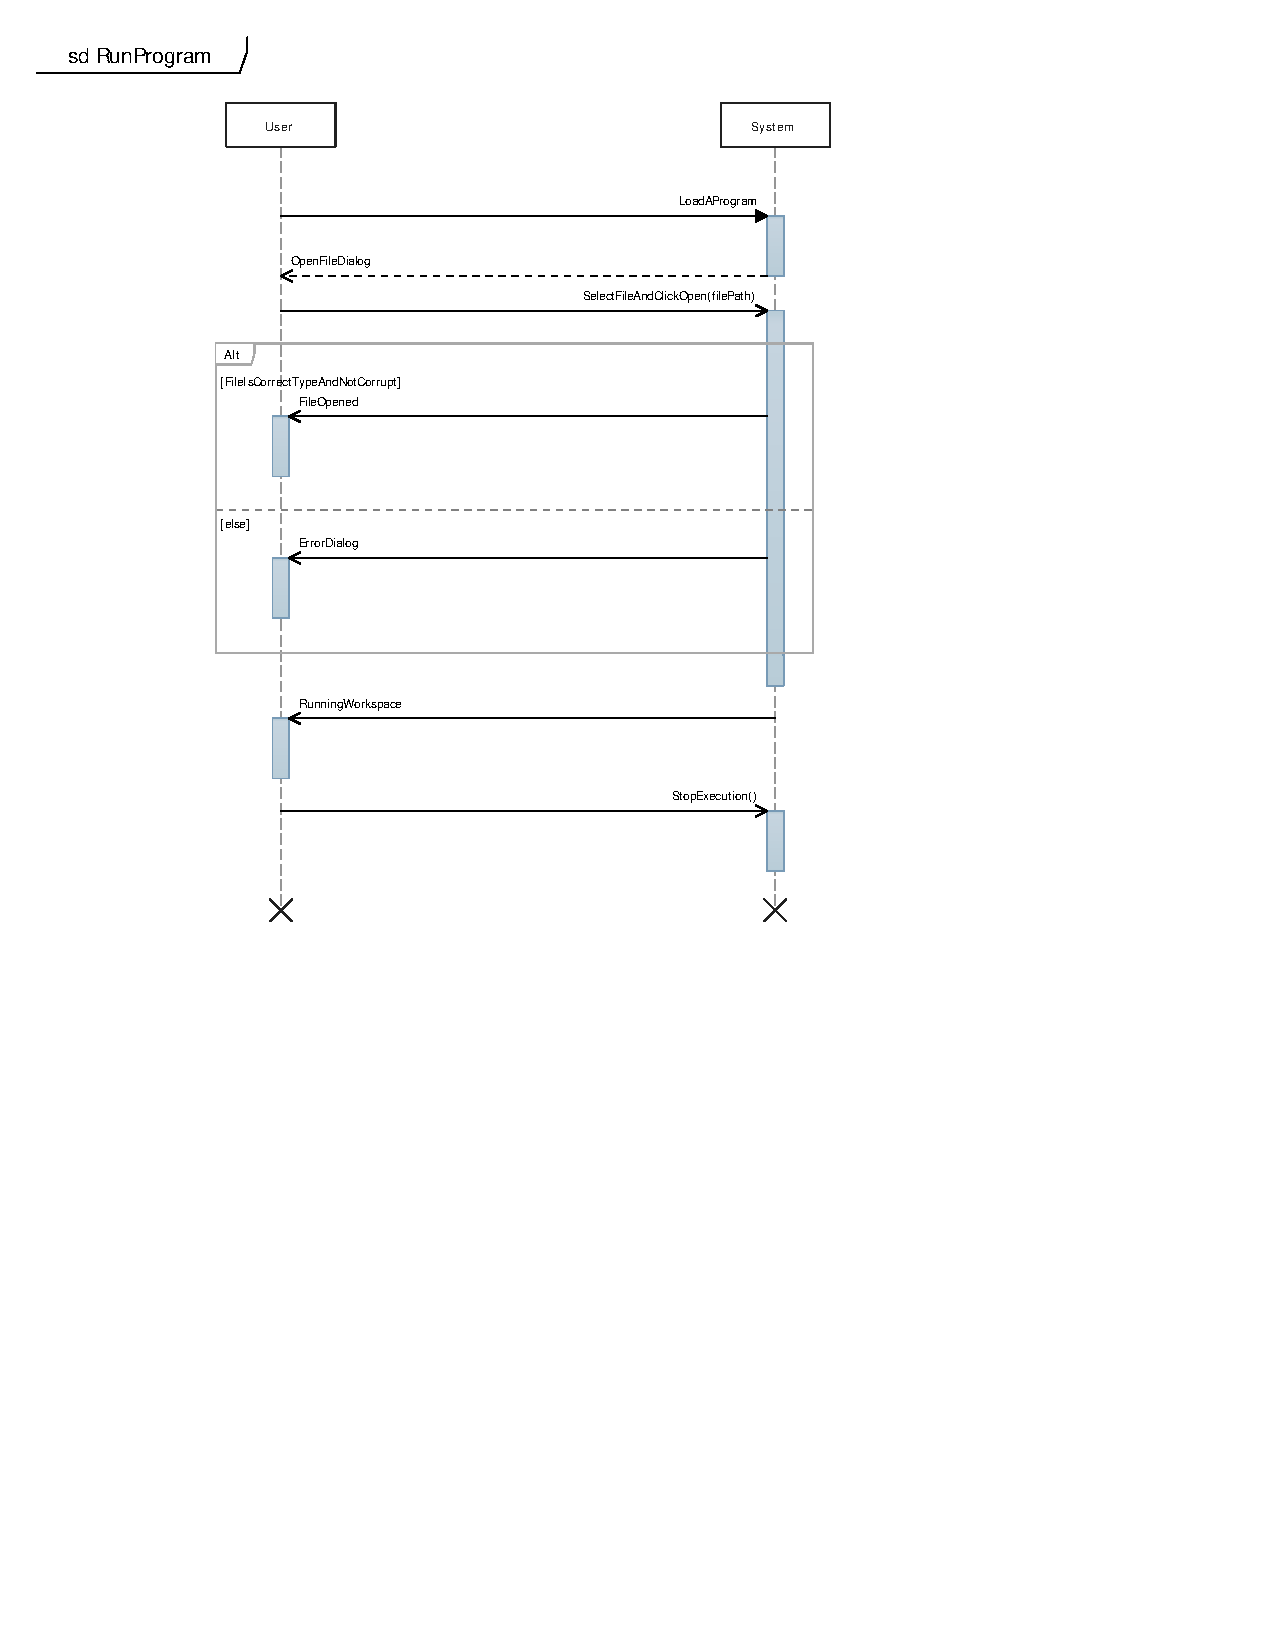
\includegraphics[scale=.7]{./pdfs/Models/SSD - RunProgram.pdf}
\end{center}

\section{Operation Contracts}
\begin{tabular*}{\textwidth}{r | l}
  \multicolumn{2}{l}{\textbf{OC1: SelectFileAndClickOpen}} \\ \hline
  \textbf{Operation} & SelectFileAndClickOpen(filePath : String) \\
  \textbf{Cross-references} & UC1: Load  program, UC2: Reload program \\
  \textbf{Preconditions} & The OpenFileDialog is open. \\
  \textbf{Post-conditions} & The file name was parsed. \\
                            & The emulator opened the file. \\ \hline
\end{tabular*} \\\\

\begin{tabular*}{\textwidth}{r | l}
  \multicolumn{2}{l}{\textbf{OC2: ZoomSliderChanged}} \\ \hline
  \textbf{Operation} & ZoomSliderChanged(zoomLevel : int) \\
  \textbf{Cross-references} & UC3: Zoom screen \\
  \textbf{Preconditions} & There is an application running in the workspace. \\
  \textbf{Post-conditions} & The workspace canvas has been magnified appropriately. \\
                           & The workspace zoomLevel attribute was updated. \\ \hline
\end{tabular*} \\\\

N.B. Additional operation contracts for the remaining use cases were not pursued because of their similarly trivial nature. The basic format of this operation contract --- user changes UI element, UI adjusts accordingly, and program updates relevant attributes --- applies to the other use cases.

\section{Design Class Diagram}
\begin{center}
        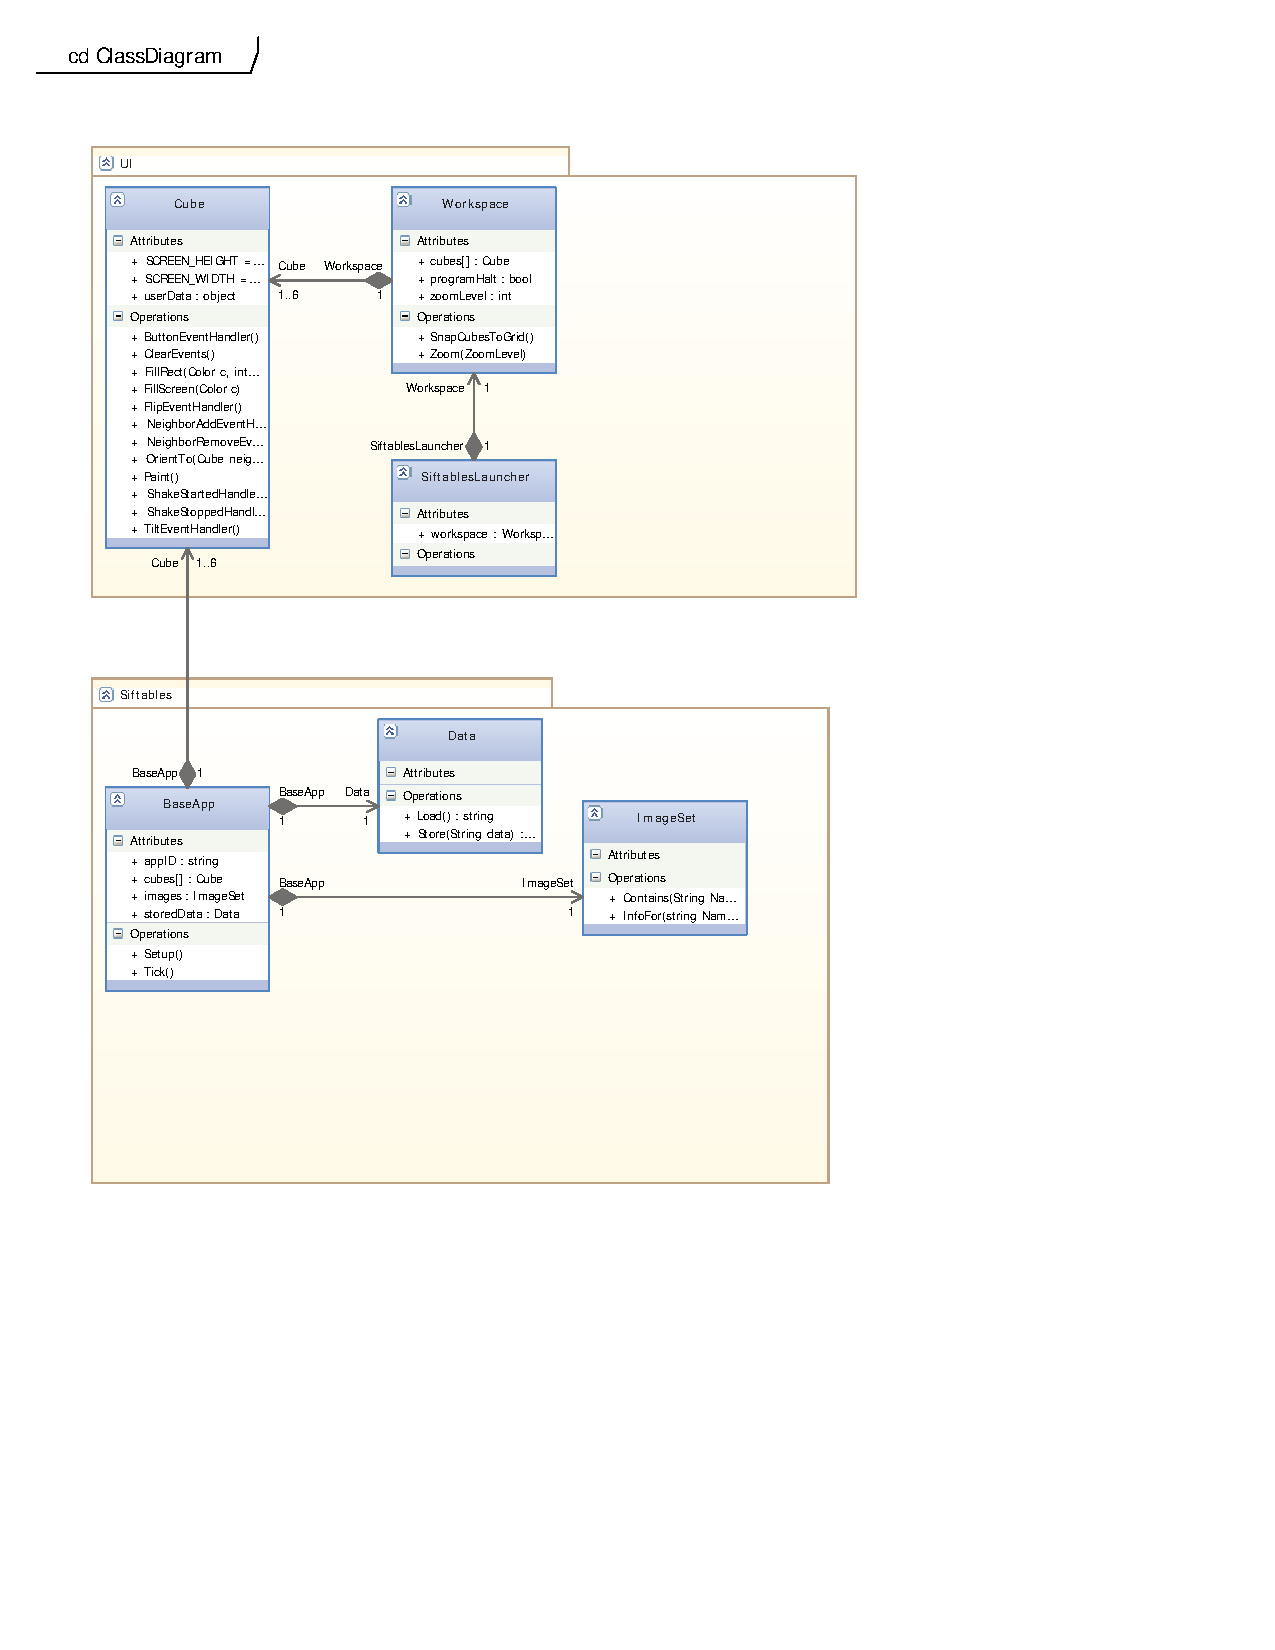
\includegraphics{./pdfs/Models/Class Diagram.pdf}
\end{center}

\section{Sequence Diagrams}
\begin{center}
        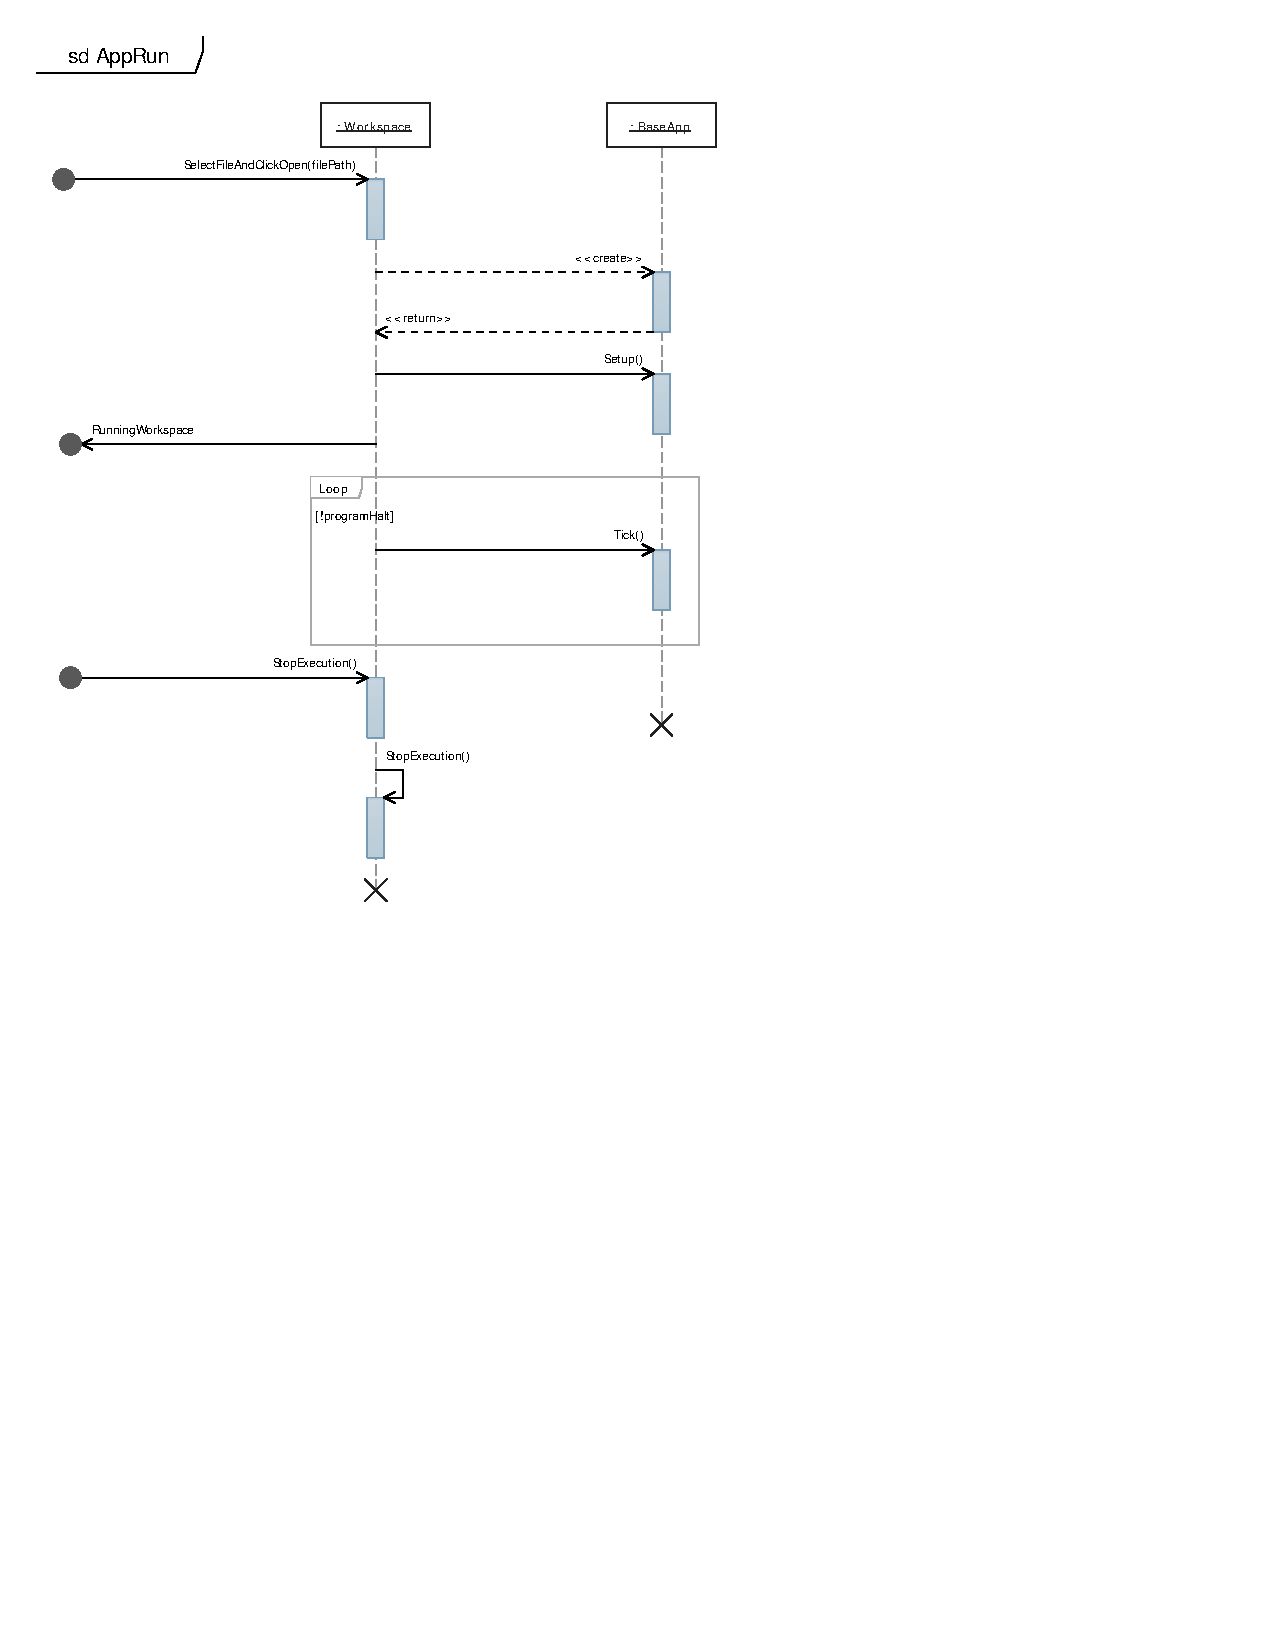
\includegraphics{./pdfs/Models/SD - AppRun.pdf}
        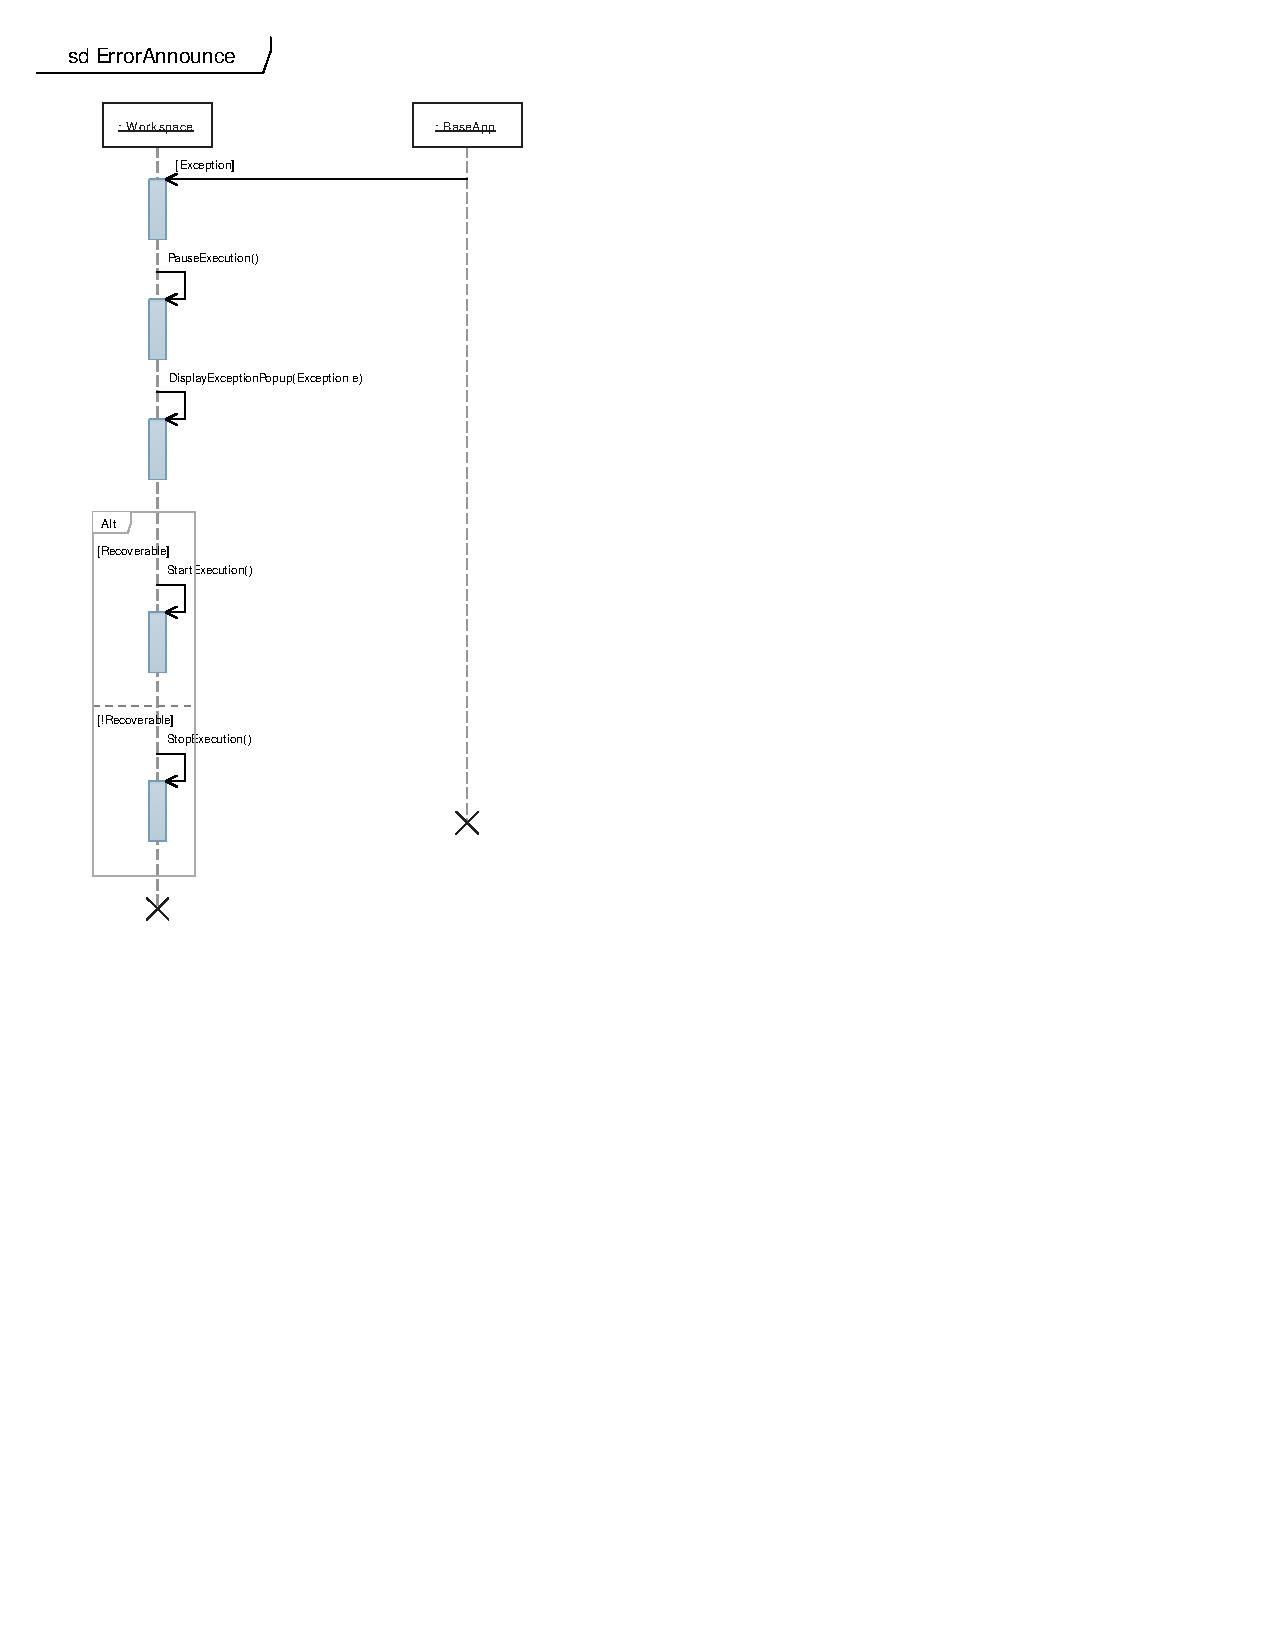
\includegraphics{./pdfs/Models/SD - ErrorAnnounce.pdf}
\end{center}
        
\end{document}
